\section{Cylindrical Detector System}

The cylindrical detector system (CDS) surrounds the experimental target system to measure produced charged particles.
The CDS consists of three parts, the outermost part is the solenoid magnet to make the uniform magnetic field for momentum analysis,
next is the cylindrical detector hodoscope (CDH) to measure time-of-flight from the T0 and make trigger signal,
and the cylindrical drift chamber (CDC) to measure the trajectory in the magnetic field, by which the momentum of a charged particle is analyzed.
Particle identification is performed by the momentum and T0-CDH TOF.

\subsection{Solenoid magnet}
\begin{frame}{CDC fine turning}
  \begin{tabular}{cc}
    \begin{minipage}{0.5\hsize}
      \begin{figure}
        Before\\
        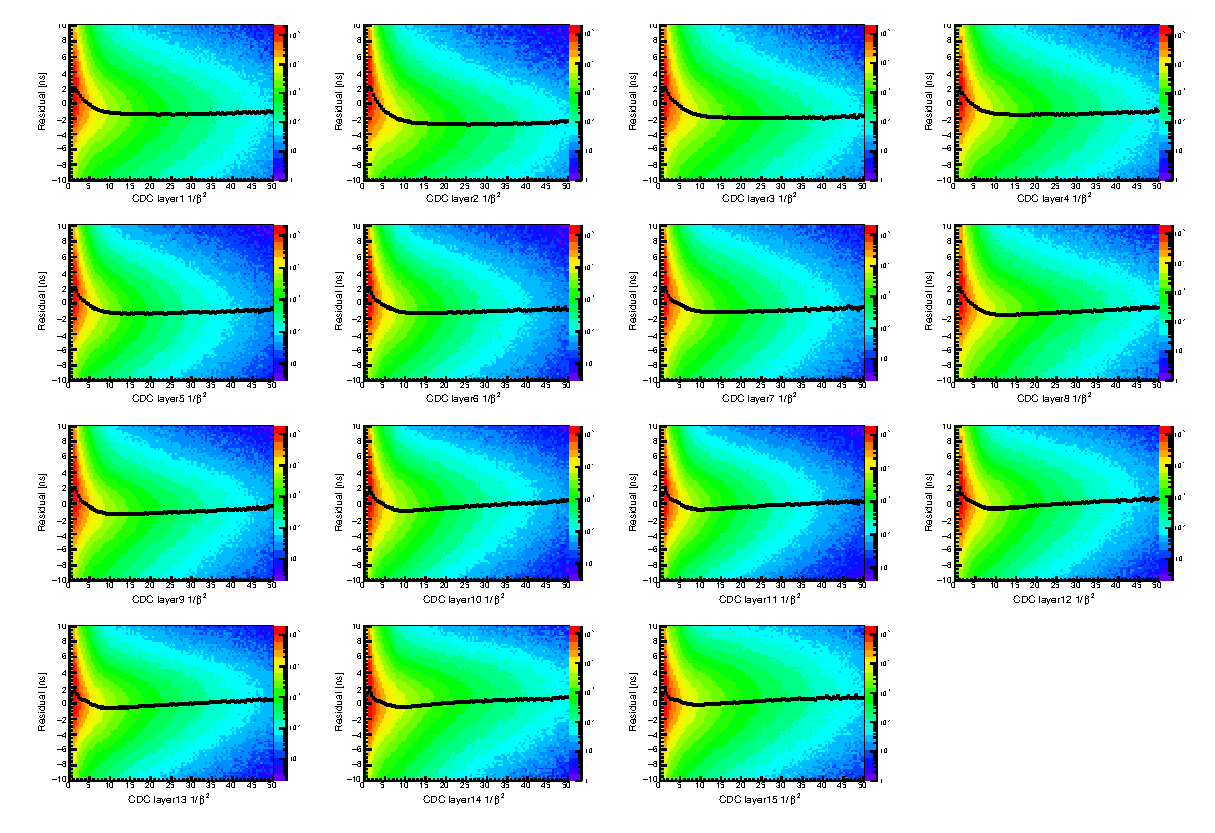
\includegraphics[width=5cm]{../pic/Run78/CDS/CDC_ob2_res_before.eps}
      \end{figure}
    \end{minipage}

    \begin{minipage}{0.5\hsize}
      \begin{figure}
        After\\
        \includegraphics[width=5cm]{../pic/Run78/CDS/CDC_ob2_res.eps}
      \end{figure}
    \end{minipage}
  \end{tabular}
  \centering
  $\beta$ and residual has correlation, which was calibrated wire-by-wire.
\end{frame}

\begin{frame}{Vertex image by CDS and BPC}
  \begin{figure}
    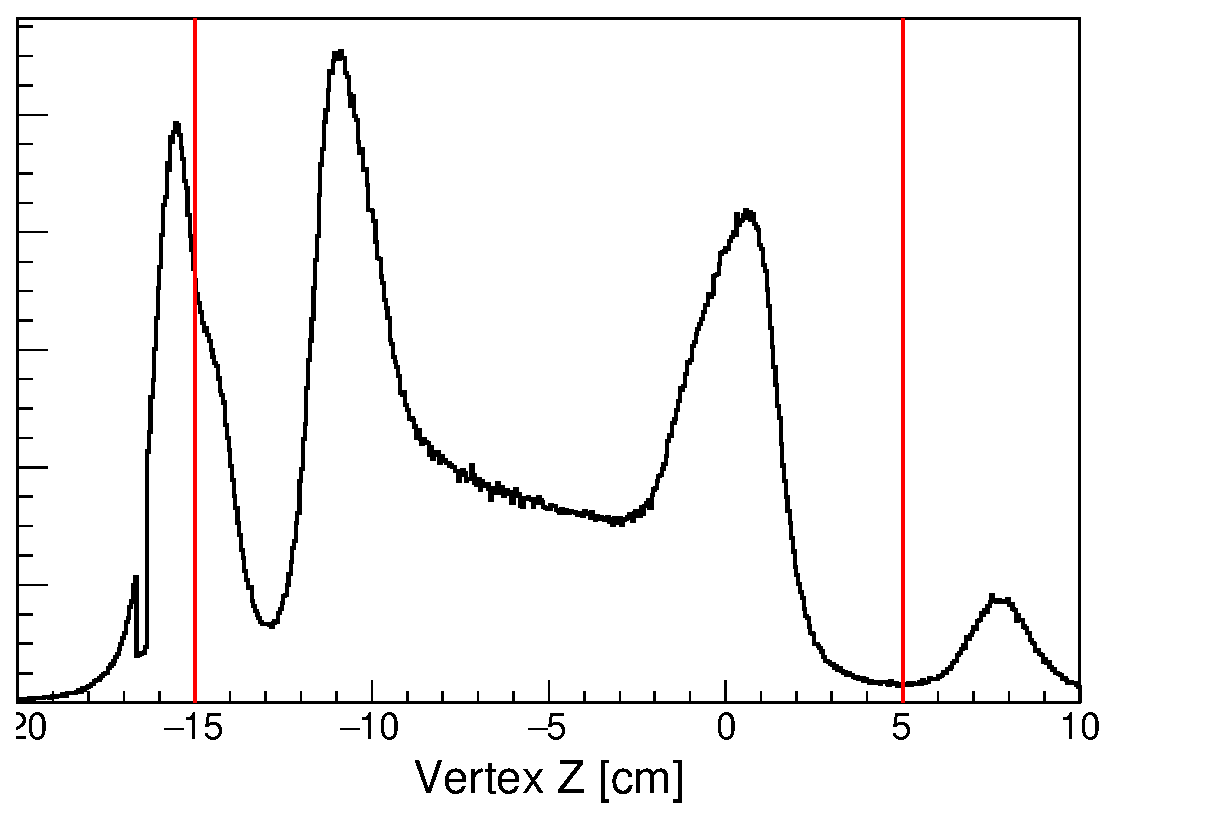
\includegraphics[width=8cm]{../pic/Run78/CDS/vertex.eps}
  \end{figure}
\end{frame}

\begin{frame}{Vertex image by CDS and BPC (Vertex cut)}
  \begin{figure}
    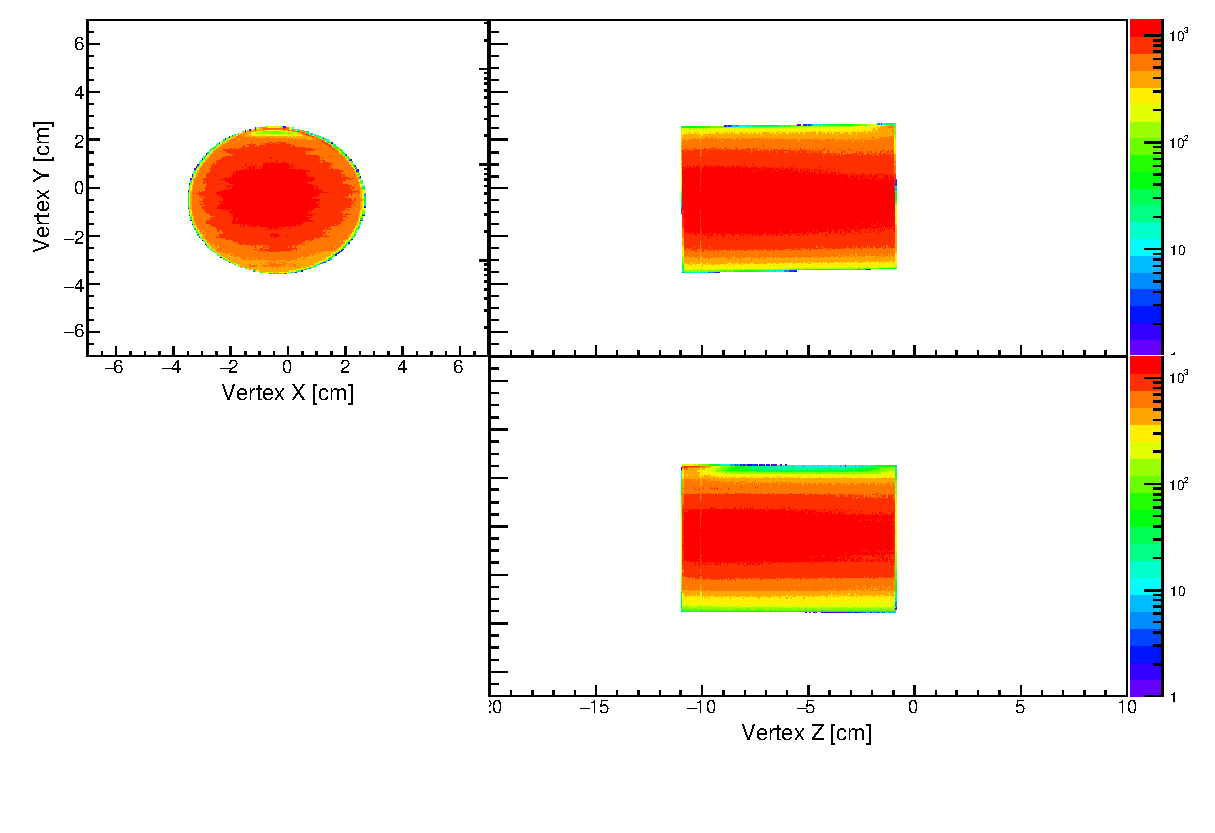
\includegraphics[width=8cm]{../pic/Run78/CDS/vertex_f.eps}
  \end{figure}
\end{frame}

\begin{frame}{Vertex resolution}
  \begin{tabular}{cc}
    \begin{minipage}{0.5\hsize}
      \begin{figure}
        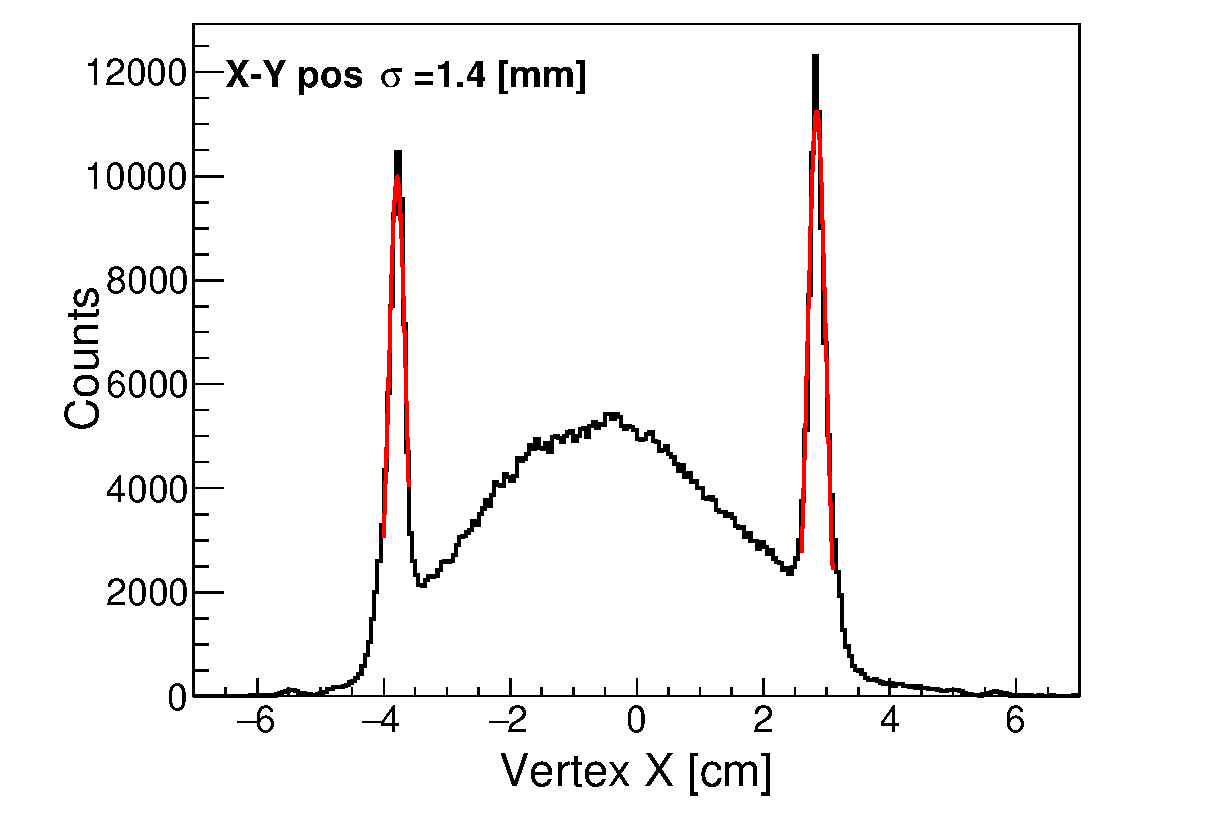
\includegraphics[width=5cm]{../pic/Run78/CDS/vertex_x.eps}
      \end{figure}
      \centering
      Y range was selected \\ $-5.5\sim-5$ [mm]
    \end{minipage}

    \begin{minipage}{0.5\hsize}
      \begin{figure}
        \includegraphics[width=5cm]{../pic/Run78/CDS/vertex_z.eps}
      \end{figure}
      \centering
      $Z =0$ was selected [mm]\\
      resolution was evaluated by DEF.
    \end{minipage}
  \end{tabular}
\end{frame}

\begin{frame}{CDS mass$^2$ vs momentum}
  \begin{figure}
    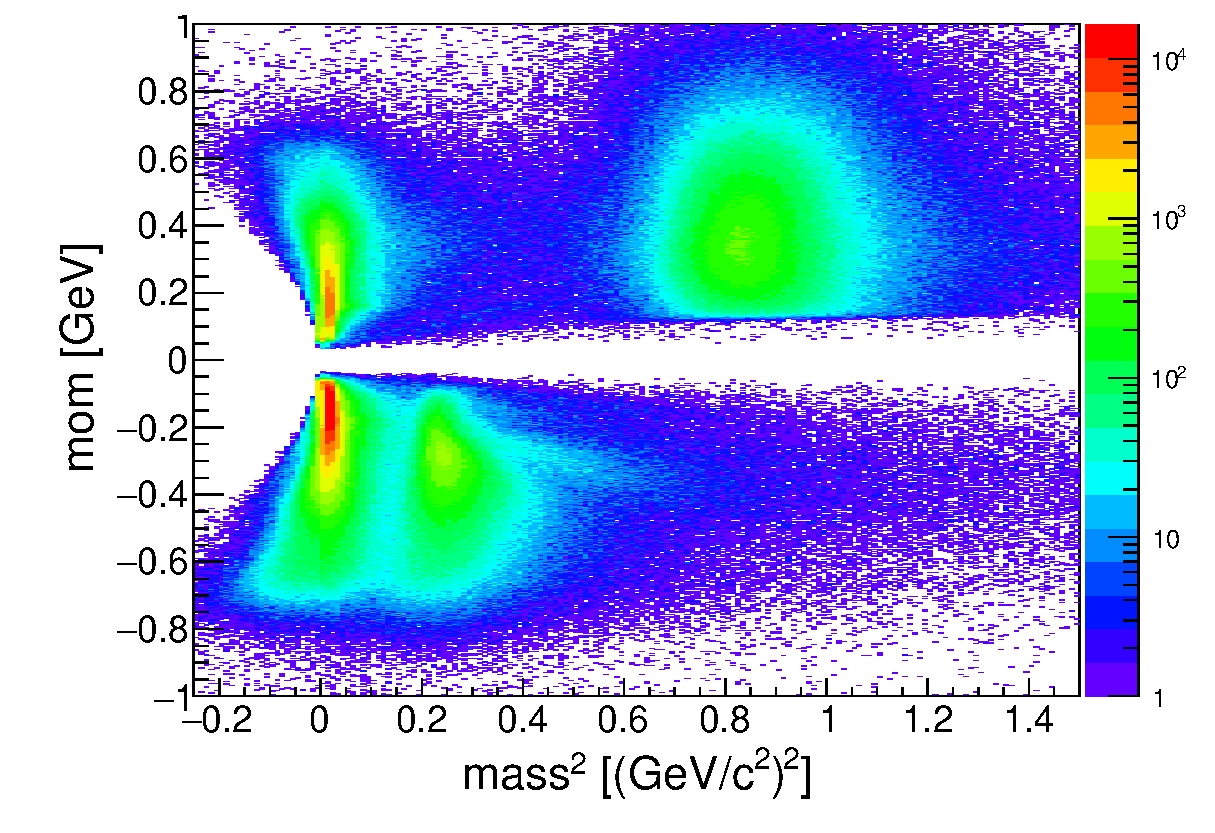
\includegraphics[width=8cm]{../pic/Run78/CDS/pid.eps}
  \end{figure}
\end{frame}

\begin{frame}{Invaraint mass by CDS}
  \begin{tabular}{cc}
    \begin{minipage}{0.5\hsize}
      \begin{figure}
        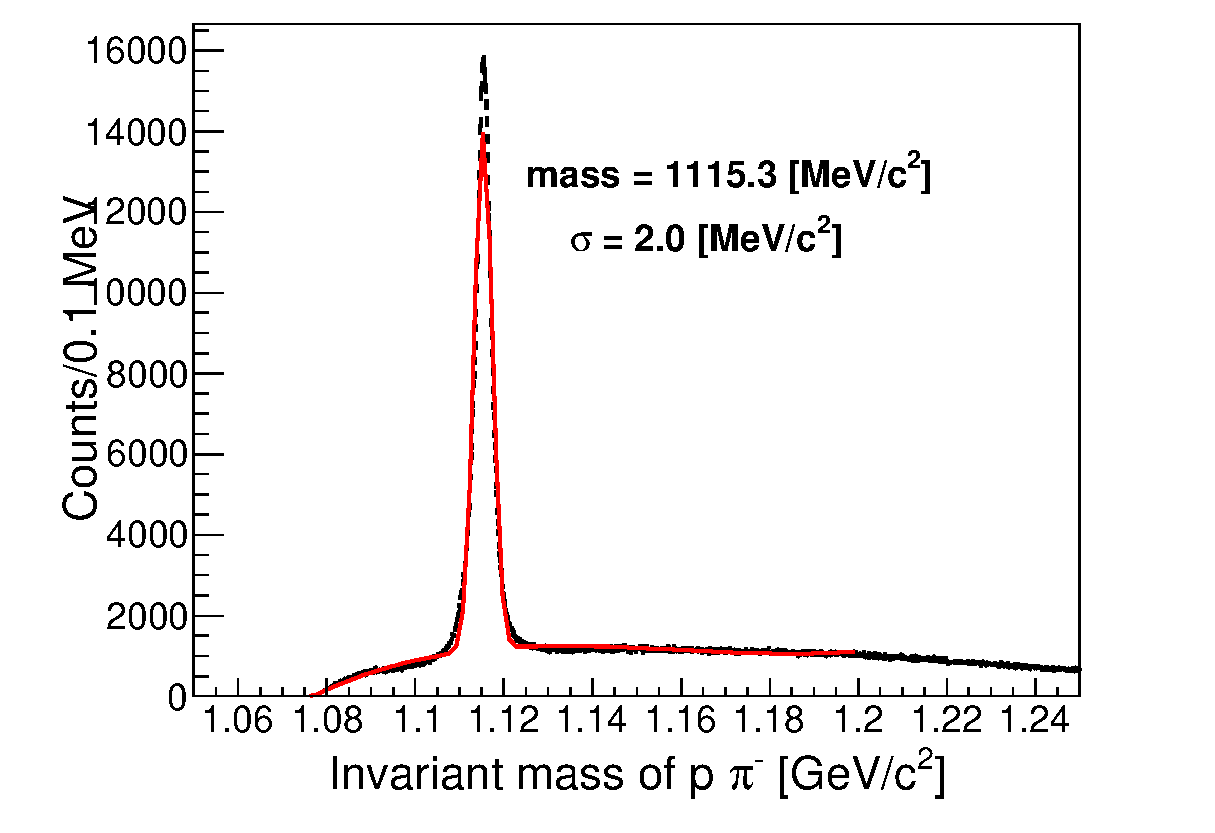
\includegraphics[width=5cm]{../pic/Run78/CDS/IM_ppim.eps}
      \end{figure}
    \end{minipage}

    \begin{minipage}{0.5\hsize}
      \begin{figure}
        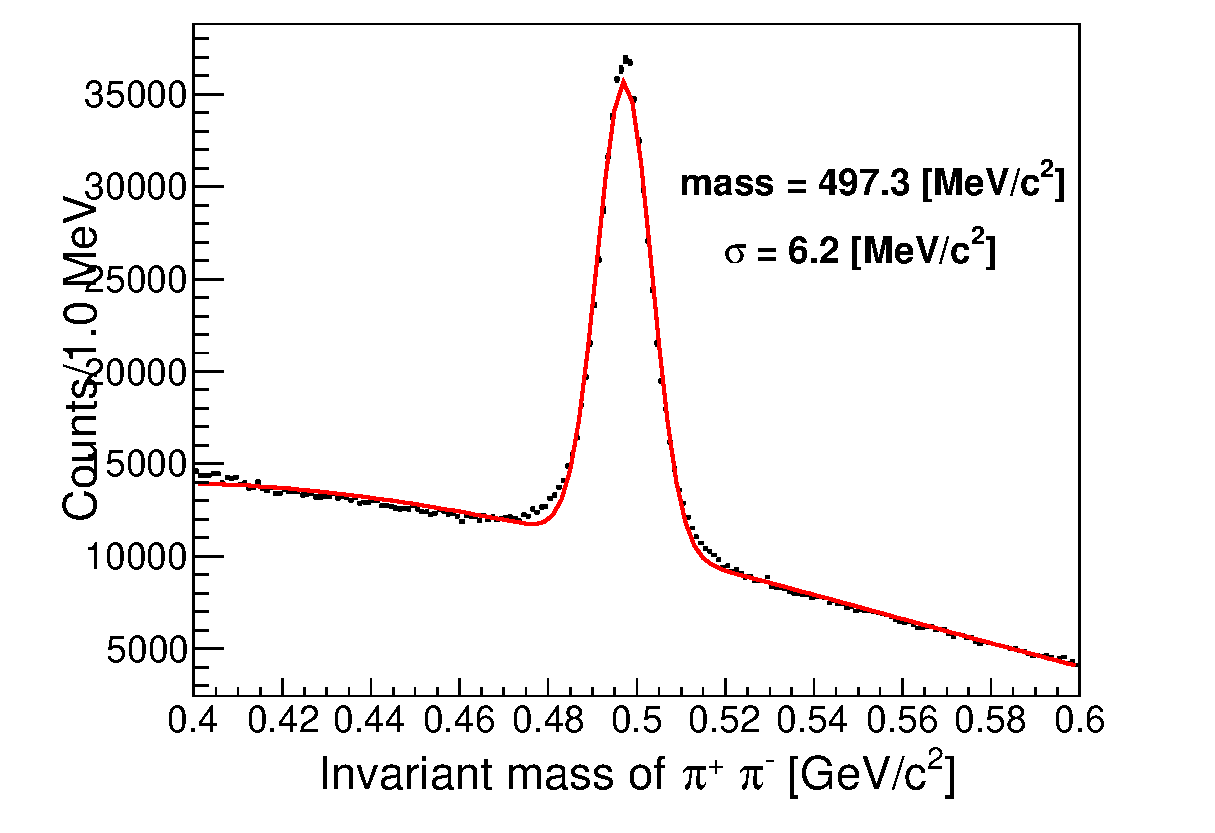
\includegraphics[width=5cm]{../pic/Run78/CDS/IM_pipi.eps}
      \end{figure}
    \end{minipage}
  \end{tabular}
\end{frame}




The CDS is a solenoid type spectrometer whose bore diameter is 1.18m and the length is 1.17m with an overall weight is about 23 tons.
The design of the solenoid magnet is shown in Fig\ref{fig:CDS_solenoid}.
The magnet provides a uniform field strength inside the tracking volume, 420mm front to back from the center.
In the present experiment, it is operated at 0.7T.

\begin{figure}[htbp]
  \centering
  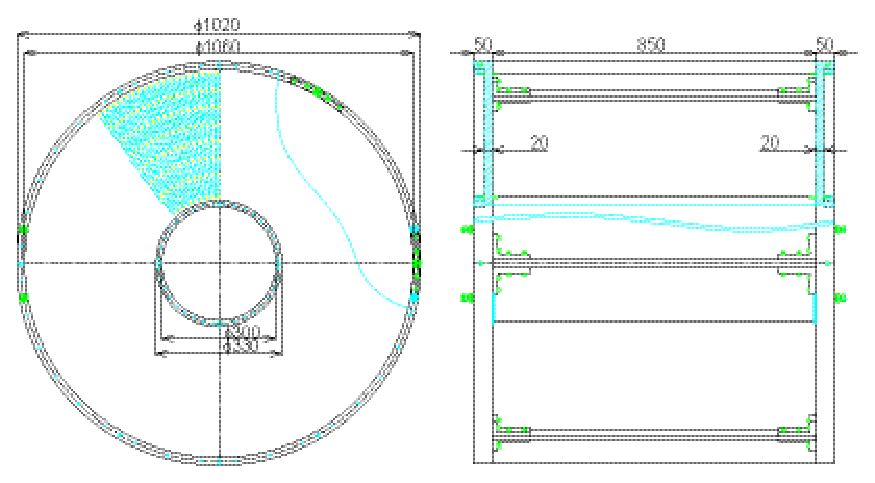
\includegraphics[width=10cm]{pic/experiment/CDC_structure.eps}
  \caption{
    Design of the CDC (all dimensions in mm).
    The CDC consists of two aluminum end-plates, a 1mm thick CFRP cylinder as an inner wall, and six aluminum posts that are placed outside the tracking volume.
  }
  \label{fig:CDC_structure}
\end{figure}

\subsection{Cylindrical Detector Hodoscope - CDH}
The CDH is a segmented plastic scintillation counter used for the charged particle trigger and particle identification.
The CDH is located at a radius of 544mm from the beam axis covering a polar angle range from 54 to 126 degree corresponding to a solid angle coverage of 59$\%$ of 4$\pi$.

The CDH consists of 36 modules, individually mounted on the inner wall of the solenoid magnet.
The scintillators are mode of ELJEN EJ-200, with dimensions of 790mm in length, 99mm in width, and 30mm in thickness.
The scintillation light is transferred through light guides to a pair of Hamamatsu R7761 fine-mesh 19-dynode photomultipliers 1.5 inches in diameter.

The CDH is operated in the 0.7T magnetic field with a typical PMT gain of $\sim 10^6$.
The measured average time resolution of the CDH without a magnetic field is $71\pm3$ ps ($\sigma$), obtained with cosmic ray data. The error represents the variation among the segments.


\subsection{Inner Hodoscope - IH}
The inner hodoscope (IH) is a segmented plastic scintillation counter mounted on the inner wall of the CFRP cylinder of the CDC at a radius of 140mm from the beam axis.
The IH consists of 24 ELJEN EJ-200 scintillators with a dimension of 600mm in length, 27mm in width, and 3mm in thickness.
Each segment is overlapped by 1mm due to the strong magnetic field and limited space.
Readout uses the multi-pixel photon counters (MPPCs) with a 3mm $\times$ 3mm sensitive area (Hamamatsu S10362-33-100C), which is attached only upstream side.
The scintillation light is collected by 4 wavelength-shifting fibers embedded in the scintillator and connected to an MPPC with a specially designed connector.
The MPPC signal is read out by using a preamplifirer.

The IH was used as a trigger counter for the efficiency estimation of the CDC.
The IH was removed in MR RUN78 to increase acceptance for the backward scattered proton.

